\documentclass{article}
\usepackage[utf8x]{inputenc}
\usepackage{lipsum}
\usepackage[margin=1in,includefoot]{geometry}
\usepackage{fancyhdr}
\pagestyle{fancy}
\usepackage{pifont}
\newcommand{\cmark}{\ding{51}}
\newcommand{\xmark}{\ding{55}}
\usepackage{listings}
\usepackage{color}
\usepackage{hyperref}
\usepackage[table]{xcolor}
\usepackage{graphicx}
\usepackage{float}
\usepackage{longtable}
\usepackage[T1]{fontenc}
\usepackage{textcomp}
\usepackage[english]{babel}
\usepackage[T1]{fontenc}
\usepackage{uarial}
\renewcommand{\familydefault}{\sfdefault}
\definecolor{dkgreen}{rgb}{0,0.6,0}
\definecolor{gray}{rgb}{0.5,0.5,0.5}
\definecolor{mauve}{rgb}{0.58,0,0.82}
\hypersetup{
    colorlinks=true, % make the links colored
    linkcolor=black, % color TOC links in blue
    urlcolor=blue, % color URLs in red
    linktoc=all % 'all' will create links for everything in the TOC
}
\lstset{
    commentstyle = \color{gray},
    extendedchars = \true,
    inputencoding = utf8x,
    language = php,
    keepspaces = true,
    keywordstyle = \bfseries,
    backgroundcolor = \color{blue!25},
    xleftmargin = 2cm,
    framexleftmargin = 1em
}

\begin{document}
\rowcolors{2}{teal!20}{white}
\begin{titlepage}
\begin{center}
\begin{figure}[H]
\centering
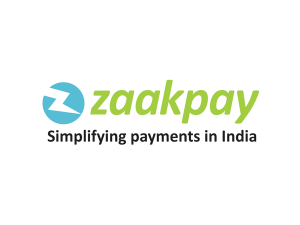
\includegraphics[width=2.8 in]{306.png}
\end{figure}
\line(1,0){350}\\
\huge{\bfseries Zaakpay UPI Integration Document}
\line(1,0){250}\\
[1.5cm]
\textsc{\Large Version 1.0}
\end{center}


\end{titlepage}
\section{Staging Credentials}
\begin{itemize}
\item {\bfseries URL : } http://zaakpay-staging.cloudapp.net:8080
\item {\bfseries Merchant Identifier :} b19e8f103bce406cbd3476431b6b7973
\item {\bfseries Secret key :} 0678056d96914a8583fb518caf42828a
\end{itemize}

\newpage
\section{Request and Response}
\subsection{Production URL}
\begin{itemize}
\item {\bfseries PCI-DSS certified merchants:}\\
In this case, the Transact URL will be: {\bfseries https://api.zaakpay.com/transactD?v=5}\\ Here the card details will be encrypted on the merchant's server using RSA encryption.
\item {\bfseries PCI-DSS non-certified merchants:}\\
In this case, the Transact URL will be: {\bfseries https://api.zaakpay.com/transactD?v=3}\\ Here the card details will be encrypted on Zaakpay's server using a js file.

\end{itemize}
\subsection{Request Parameters}
\begin{longtable}{||c|| p{2.09cm}|| p{5.5cm} || p{4.7cm}||}
\rowcolor{white}

\caption{S2S API Request}\\
 \rowcolor{green!50}
\bfseries{Parameter} & \bfseries{Optional O, Mandatory M} & \bfseries{Validation} & \bfseries{Allowed Values} \\ \hline
merchantIdentifier & M & alphanumeric & Zaakpay's unique identifier for your website \\
orderId & M & max 20 alphanumeric,must be unique per website, we do not accept duplicate & Your unique transaction identifier. \\
returnUrl & O & This must be the domain(or a sub-domain of it) you saved under My Account>Integration & Url where you want Zaakpay to post the response \\
buyerEmail & M & valid email address of the buyer & eg. prasang.misra@mobikwik.com \\
buyerFirstName & M & Max 30 alphanumeric characters, no special characters or dashes. First Name on card & Prasang \\
buyerLastName & M & Max 30 alphanumeric characters, no special characters or dashes. First name and last name cannot be same. Last Name on card. & Misra \\
buyerAddress & M & 100 alphanumeric Street address of the buyer. (Part of billing address) & B-34, Priyadarshni Society, Dumna Road \\
buyerCity & M & 30 alphabet, minimum 3 (Part of billing address) & Jabalpur \\
buyerState & M & State of the buyer (Part of billing address) & MP \\
buyerCountry & M & Country of the buyer & India\\
buyerPincode & M & Buyer's pin/zip code. Can have Numbers,
Spaces and Hyphens (-)only ( Part of billing address ) & 482001 \\
buyerPhoneNumber & M & buyer's landline or mobile phone number, numeric only, no dashes,no spaces & eg. 7698189874 \\
txnType & M & 1 digit only, numeric Zaakpay will show the tab on the payment page which corresponds to the txnType you provide & For UPI, it is 3 \\
zpPayOption & M & Which Zaakpay option have you used for this transaction. 1 digit only, numeric Default value is 1. & For UPI, it is 3 \\
mode & M & 1 digit only, numeric & 1 = Domain check, 0=Domain check skip\\
currency & M & Values defined by Zaakpay & INR\\
amount & M & Value in paisa. Min 100 paisa Max 10000000. Amount limit saved under Transaction Limit in your Zaakpay panel. & \\
merchantIpAddress & M & buyer's IP address as recorded by your website. & 127.0.0.1 \\
txnDate & M & Transaction date in yyyy-mm-dd format & Eg. 2016-08-20 \\
purpose & M & Min and max numeric 1 digit. You must specify the purpose of the transaction & 0=Service, 1=Goods, 2=Auction, 3=Other\\
productDescription & M & Text description of what you are selling. Atleast 1 product description is mandatory to show in the bill on payment page. free text alphanumeric 100 max & e.g. name of book, name of mobile etc. e.g. Rs 199 Godzilla Movie DVD \\
product1Description & O & free text alphanumeric 100 max & \\
product2Description & O & free text alphanumeric 100 max & \\
shipToAddress & O & You may specify this only when buyer's address is different from shipping address. 30 alphanumeric & Flat 1A, Sector7, Defence Colony \\
shipToCity & O & Shipping address city. 30alphabet, minimum3 & Jabalpur \\
shipToState & O & Shipping address state & MP \\
shipToCountry & O & Shipping address country & India \\

shipToPincode & O & Shipping address pin/zip code. 2 to 12 digits Can have Numbers, Spaces and Hyphens (-)only & 482001\\
shipToPhoneNumber & O & Shipping address landline or mobile phone number numeric only, no dashes,no spaces & e.g. 01145771775 ,9971712962\\
shipToFirstname & O & max 30 alphanumeric characters,no  special characters or dashes & Prasang\\
shipToLastname & O & max 30 alphanumeric characters,no  special characters or dashes & Misra\\
showMobile & O & false:We show the full-fledged version unconditionally. DETECT:We do detection of the user Agent of the browser from which the request is sent\& route accordingly. true:We show the mobile page unconditionally. missing/not sent: Same as DETECT (i.e. We do detection at our end ). & Only allowed value is “true” if you want Zaakpay to represent mobile view.\\
debitorcredit & M & Possible Value: UPI & \\
bankid & M  & VPA address of the customer & \\
checksum & M & To be calculated on above parameters using HMAC SHA 256 & \\
\end{longtable}

The card details need to be encrypted and sent across the https POST parameters. This encryption can be done by the help of RSA encryption.
Example:
Since you are sending payment information to Zaakpay, you need to pre-fill form parameters as hidden
fields as a part of a form. Here is an example of what a form sending information to Zaakpay looks
like:

\begin{lstlisting}[language=html,breaklines=true]
<form action="https://api.zaakpay.com/transactD?v=3" method="post">
<input type="hidden" name="merchantIdentifier" value="b19e8f103bce406cbd">
<input type="hidden" name="orderId" value="444221414">
<input type="hidden" name="returnUrl" value="">
<input type="hidden" name="buyerEmail" value="a@b.com">
<input type="hidden" name="buyerFirstName" value="Prasang">
<input type="hidden" name="buyerLastName" value="Misra">
<input type="hidden" name="buyerAddress" value="JBP">
<input type="hidden" name="buyerCity" value="Jabalpur">
<input type="hidden" name="buyerState" value="M.P.">
<input type="hidden" name="buyerCountry" value="India">
<input type="hidden" name="buyerPincode" value="482001">
<input type="hidden" name="buyerPhoneNumber" value="7698189874">
<input type="hidden" name="txnType" value="3">
<input type="hidden" name="zpPayOption" value="3">
<input type="hidden" name="mode" value="0">
<input type="hidden" name="currency" value="INR">
<input type="hidden" name="amount" value="200000">
<input type="hidden" name="merchantIpAddress" value="127.0.0.1">
<input type="hidden" name="purpose" value="1">
<input type="hidden" name="productDescription" value="test product">
<input type="hidden" name="product1Description" value="">
<input type="hidden" name="product2Description" value="">
<input type="hidden" name="product3Description" value="">
<input type="hidden" name="product4Description" value="">
<input type="hidden" name="shipToAddress" value="">
<input type="hidden" name="shipToCity" value="">
<input type="hidden" name="shipToState" value="">
<input type="hidden" name="shipToCountry" value="">
<input type="hidden" name="shipToPincode" value="">
<input type="hidden" name="shipToPhoneNumber" value="">
<input type="hidden" name="shipToFirstname" value="">
<input type="hidden" name="shipToLastname" value="">
<input type="hidden" name="txnDate" value="2011-08-30">
<input type="hidden" name="debitorcredit"value="UPI" />
<input type="hidden" name="bankid" value="prasang@upi" />
<input type="hidden" name="checksum"
value="796d672eb63e1dfa4a0bc844e8d3468ebcd6d612dc39588814b7b00ce669c1c2">
</form>
\end{lstlisting}


\subsection{Response Parameters}

\begin{longtable}{||c|p{12.5cm}||}
       \caption{S2S API Response}\\
   \rowcolor{green!50}
\bfseries{Parameters} & \bfseries{Description} \\ \hline
orderId & Your unique transaction identifier \\
responseCode & Numeric, max 3 digits example 100 for success\\
responseDescription & Alphanumeric max 30 description of the response\\
amount & Txn amount in paisa, Integer \\
paymentMethod & Payment Method ID for Card and Net Banking transactions. For Card txns, payment Method ID starts with C and N for Net Banking. It is alphanumeric value with max length 6. First letter is C or N, followed by 5 digits max.\\
cardhashid & Unique id for each card number used in transaction. For Netbanking txns, value will be “NA”.\\
checksum & Checksum calculated by Zaakpay on all above response
parameters


\end{longtable}
\begin{itemize}
\item {\bfseries paymentMethod}: This parameter helps in determining the mode of payment. This parameter returns a unique id which is mapped to different cards/banks. For example, if the value of this parameter is N1001, payment was made using HDCF NetBanking. If the value is C4300, payment was made using Axis VISA Debit Card.
In case of Mobikwik Wallet, value of this parameter is N1053.
\item {\bfseries cardhashid}: This is a one to one mapping with a card number. It is a unique value generated per card and will remain same for all transactions made using same card. This can help a merchant to extract information like how many transactions and of how much worth were made using a card.  Merchants can also setup some fraud checks and limits per  card using this parameter. In case of NetBanking and Mobikwik Wallet, value of this parameter is NA. 
\item {\bfseries checksum}: Similar to request checksum, response checksum must be calculated on all response parameters by merchant and matched with the checksum sent by Zaakpay in response. Sample code to calculate response checksum has been given in file test\_merchant\_output.jsp
\end{itemize}

\end{document}
